\section{Case: FORESEE}

\subsection{Dataset}

For our second case, we use the \acrshort{foresee} dataset from the the PubDAS collections, as mentioned in Section \ref{back:relwork}. This dataset contains signals from an area around Pennsylvania in the Valley and Ridge Appalachians region, as seen in Figure \ref{fig:foresee} \cite{se-12-219-2021}. \\

\begin{figure}[!h]
    \centering
    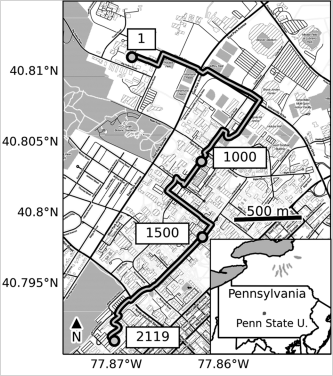
\includegraphics[width=0.5\linewidth]{figures/foresee.png}
    \caption{Map of the FORESEE Array. Source: \cite{spica2023pubdas}}
    \label{fig:foresee}
\end{figure}

\subsubsection{Data Preprocessing}
\label{exp:fordata}

\begin{table}[!h]
    \centering
    \small
    \begin{tabular}{@{}p{0.3\textwidth}p{0.3\textwidth}p{0.3\textwidth}@{}}
        \toprule
        \textbf{Parameter} & \multicolumn{2}{l}{\textbf{Value}} \\
        \midrule
        Experiment & \multicolumn{2}{l}{Foresee}  \\
        Gauge length & \multicolumn{2}{l}{\qty{10}{\si{\meter}}} \\
        Cable length & \multicolumn{2}{l}{\qty{23300}{\si{\meter}}} \\
        Channel spacing & \multicolumn{2}{l}{\qty{2}{\si{\meter}}} \\
        \midrule
        & \textbf{Original Data} & \textbf{After Preprocessing} \\
        \cmidrule(lr){2-3}
        Format & TDMS & HDF5 \\
        Sample rate & \qty{500}{\si{\hertz}} & \qty{125}{\si{\hertz}} \\
        Time window & \qty{10}{\si{\minute}} & \qty{5}{\si{\second}} \\
        Data shape & 300000 \(\times\) 2137 & 625 \(\times\) 2137 \\
        Datatype & Float32 & Float32 \\
        File size & \qty{2.5644}{\si{\giga\byte}} & \qty{4.98}{\si{\mega\byte}} \\
        \midrule
        \textbf{Dataset Information} & \multicolumn{2}{l}{} \\
        Train dataset size & \multicolumn{2}{l}{\qty{25690}{files}} \\
        Train dataset span & \multicolumn{2}{l}{2020-03-02 08:10:15 to 2020-03-03 20:40:10} \\
        Anomalous dataset size & \multicolumn{2}{l}{\qty{600}{files}} \\
        Anomalous dataset span & \multicolumn{2}{l}{2019-04-15 03:17:35 to 2019-04-15 04:07:30} \\
        \bottomrule
    \end{tabular}
    \caption{\acrshort{foresee} Experiment Data Summary}
    \label{tab:foresee_experiment_data}
\end{table}

Preprocessing of the dataset has already been performed, as detailed in the Appendix in Code Listing \ref{code:pubdas}. The files have been converted to the \acrshort{hdf5} format, and the data resampled. Due to memory constraints of most consumer-grade \acrshort{gpu}s, which typically have around 8-32GB of \acrshort{vram}, the number of 10-minute data batches that can be processed simultaneously is limited. This constraint is worsened by the need to further store the model's weights, biases, and computed losses in \acrshort{vram}. To address these limitations and enhance the system's responsiveness, we chose to split the files into 5-second segments instead of the original 10-minute recordings. This approach offers several major advantages, including:

\begin{itemize}
    \item It allows for training across various hardware architectures, accommodating different memory capacities.
    \item It enables and promotes more frequent updates in online anomaly detection, potentially identifying anomalous events every 5 seconds, dramatically improving the system's real-time response capability.
    \item For dense autoencoders, it dramatically reduces the number of parameters required.
\end{itemize}


The file-splitting process was implemented in parallel using Julia, resulting in a collection of nearly 26,000 files for our training dataset. This preprocessing strategy mitigates hardware constraints and aligns with the requirements of real- or near-real-time anomaly detection systems, where rapid identification of anomalies is crucial. A crucial aspect of our approach concerns the composition of the training dataset:

\begin{enumerate}
    \item \textit{Precense of anomalies}: The training dataset \textit{may} contain some anomalous data. This deliberate decision reflects real-world scenarios where completely ``clean'' data is rare.
    \item \textit{Time period selection}: We attempt to mitigate this by selecting a time period with minimal documented extreme weather events, earthquakes, or other known anomalous occurrences. This approach aims to minimize, but not entirely eliminate, the presence of anomalies in the training data.
    \item \textit{Model robustness}: By including potential anomalies in the training set, we aim to examine whether our models are sufficiently robust to withstand and learn from data that may contain a small proportion of anomalous samples.
    \item \textit{Semi-supervised Anomaly Detection}: Although labeled anomalies technically place our approach in the realms of self-supervised anomaly detection, our goal is to develop models that can effectively identify anomalies despite this challenge.
\end{enumerate}

It's important to note that while data quality and quantity are paramount in deep learning, we've consciously decided to balance preprocessing effort with practical considerations. Our approach aims to reduce the time and resources spent on extensive preprocessing, reflecting real-world constraints where perfect data cleaning may not always be feasible or economically viable. Information about the data can be found in Table \ref{tab:foresee_experiment_data}. 


\subsection{Experiment \rnum{1}: Model training and Reconstruction}
In this first experiment, we train four different autoencoders and examine their reconstruction capabilities, focusing on reconstruction loss, median- and overall training time. These four models consist of a dense regular autoencoder (AE), a $\beta$-variational autoencoder ($\beta$-VAE), a convolutional autoencoder (\acrshort{cae}) and finally a $\beta$-variational convolutional model ($\beta$-CVAE). Appendix \ref{app:archs} details all the layers and parameter numbers. The AE model serves as a baseline to see if we can drastically reduce dimensionality between the input layer and the first hidden layer while still achieving satisfying reconstructions and anomaly detection metrics. Likewise, the $\beta$-\acrshort{vae} lets us compare a dense autoencoder with a \acrshort{vae} model.
Furthermore, we use two convolutional variants to compare and evaluate against their prior variants. These four models allow us to compare dense and convolutional models and regular autoencoders with variational alternatives. We use $\beta$ values to help stabilize our losses, as mentioned in Section \ref{back:vae}. The objective is to compare and see if any of these relatively smaller models can effectively be used for anomaly detection in large-scale dense-sampled \acrshort{das} data. Furthermore, we seek to understand how much of the spatial characteristics we can extract.

\begin{table}[!h]
\centering
\small
\rowcolors{2}{gray!15}{white} % Start with the second row, alternate between light gray and white
\begin{tabular}{@{}lllll@{}}
\toprule
\rowcolor{gray!30} % Darker gray for the header row
\textbf{Parameter} & \textbf{AE} & \textbf{$\beta$-VAE} & \textbf{CAE} & \textbf{$\beta$-CVAE} \\
\midrule
Files & 25600 & 25600 & 25600 & 25600 \\
Input Shape & [BS, 625 × 2137] & [BS, 625 × 2137] & [BS, 1, 625, 2137] & [BS, 1, 625, 2137] \\
Batch Size & 256 & 256 & 32 & 32 \\
Model Sizes (Float16) & 5.12 GB & 5.13 GB & 91.4 KB & 126.53 MB \\
Validation Split & 0.2 & 0.2 & 0.2 & 0.2 \\
Epochs & 200 & 200 & 200 & 200 \\
Seed & 1337 & 1337 & 42069 & 1337 \\
Loss Function & \acrshort{mse} & \acrshort{elbo} ($\beta=0.8$) & \acrshort{mse} & \acrshort{elbo} ($\beta=0.5)$ \\
Optimizer & ADAM & ADAM & ADAM & ADAM \\
Learning Rate & 0.001 & 0.001 & 0.002 & 0.001 \\
LR Scheduler & ReduceOnPlateau & ReduceOnPlateau & ReduceOnPlateau & ReduceOnPlateau \\
Early Stopping Patience & 10 & 10 & 10 & 10 \\
Early Stopping Min $\Delta$ & 0.0001 & 0.0001 & 0.0001 & 0.001 \\
\bottomrule
\end{tabular}
\caption{Hyperparameters for all models}
\label{tab:hyperparameters}
\end{table}
As shown in Table \ref{tab:hyperparameters}, we need to decrease the batch size for convolutional models since each convolutional layer operates on higher-dimensional data, increasing \acrshort{gpu} memory usage during training. Additionally, the \acrshort{vae} models require extra parameters since the latent layer is represented by both $\mu$ and $\sigma$ layers, slightly increasing their size compared to their non-variational counterparts. The convolutional models are significantly smaller overall, which is great for real-world scenarios due to possible hardware constraints. Detailed descriptions of all the models and their layer structures can be found in Appendix \ref{app:archs}. 

 The relatively large batch sizes (256 for linear models and 32 for convolutional) allow for stable gradient updates. At the same time, the learning rate of 0.001 is a common starting point for the \acrshort{adam} optimizer \cite{kingma2017adam}. To optimize the training process, we introduce a learning rate scheduler that reduces the learning rate by half if the validation loss does not decrease over 5 epochs. Combined with an early-stop mechanism, we can attempt escaping local minima during gradient descent and stop unnecessary training whenever the validation loss does not decrease by at least min $\Delta$ by 10 consecutive epochs.  

To evaluate and compare the reconstruction capabilities of these models, we will primarily use the \acrshort{mse} for the AE and CAE, and  \acrshort{elbo} loss with \acrshort{mse} for $\mathcal{L}_{rec}$ for the $\beta$-VAE and $\beta$-CVAE, as described in section \ref{back:elbo}. Common metrics like loss, inference time, training times, and epochs before the best loss will be prioritized for this experiment. Finally, we also visually inspect three reconstructed samples to assess the models' performance qualitatively.

\subsection{Experiment \rnum{2}: Anomaly Detection}

For this experiment, we select a test dataset for labeling anomalies based on the findings of Zhu et al. \cite{zhu2023seismic}, who identified 18 thunder-induced seismic events between 03:20 and 03:50 on the 15th of April 2019. Based on this, we try to label heatmaps to allow for finding a higher $\epsilon^*$. As discussed in Section \ref{back:relwork}, several studies on \acrshort{das} data concern themselves with specific events they target, such as earthquakes. Researchers have identified certain characteristics of anomalous data for the \acrshort{foresee} dataset as mentioned in Section \ref{back:relwork}. Labeling some data allows for finding a potentially better threshold, which can be done by studying how F1-score changes iteratively, as mentioned in Section \ref{back:anomdet}; what we ultimately want in a real-world scenario is to detect anomalies with as high accuracy as possible while keeping a low FPR. Our approach can thus be described as unsupervised training with supervised evaluation. To assess model performance, we use evaluation metrics presented in Section \ref{back:anomdet} to measure our models. We use single- and half-precision inference for detection to compare the results. However, ROC and PR curves will only be shown at half-precision. This experiment generally aims to compare smaller autoencoders for detecting anomalous events using a labeled dataset and compare single- and half-precision results.

\subsubsection{Experiment Setup}
Model training and anomaly detection are performed on \gls{idun}. Table \ref{tab:system-specs} in Appendix \ref{app:idun} shows details of the machines used. \\

